\documentclass[xcolor={dvipsnames},pdf, hyperref={colorlinks=true, citecolor=ForestGreen, linkcolor=BlueViolet, urlcolor=Magenta}, handout]{beamer}
\usetheme{Frankfurt}  
\usecolortheme{whale}
\usepackage{tikz} 
\usepackage{amsmath}
\usepackage{amsthm}
\usepackage{amssymb}              % used for \eqref{} in this document
\usepackage{dsfont}
\usepackage{hyperref}
\usepackage{threeparttable}
\usepackage{multirow}
\graphicspath{{Figures/}}
\usepackage{booktabs}
\usepackage{tikz}
\newtheorem{exmp}{Example}[section]
\usepackage{subcaption}
\usepackage{adjustbox}
\usepackage{graphicx}
\usepackage[mathscr]{euscript}
\usepackage{remreset}% tiny package containing just the \@removefromreset command
\makeatletter
\@removefromreset{subsection}{section}
\makeatother
\setcounter{subsection}{1}
\usepackage{float}
\usepackage{sgamevar}
\usepackage{sgame}


\newcommand{\defn}[1]{\textbf{#1}}


%Instructor version
\newcommand{\blank}[0]{}
\newcommand{\ddp}[1]{{\textcolor{ForestGreen}{#1}}} 
\newcommand{\dd}[1]{{\underline{\textcolor{ForestGreen}{#1}}}}

%Student version
%\newcommand{\blank}[0]{\vspace{2em}}
%\newcommand{\dd}[1]{\underline{\hspace{3cm}}} 
%\newcommand{\ddp}[1]{}

\addtobeamertemplate{navigation symbols}{}{%
	\usebeamerfont{footline}%
	\usebeamercolor[fg]{footline}%
	\hspace{1em}%
	\insertframenumber/\inserttotalframenumber
}

%% preamble
\title{Perfect Competition}
\author{David A. D\'iaz}
\institute{UNC Chapel Hill}
\date{}


\AtBeginSection[] %Section links on slides

\section{Introduction}

\begin{document} 
	
	\begin{frame}
		
		\titlepage
		
	\end{frame}
	

\begin{frame}{Perfect Competition}
\begin{itemize}
	\item 	Perfectly competitive markets are characterized by
	\begin{enumerate}
		\item Many buyers and sellers in the market
		\item The good/service being provided by sellers is identical
		\item Firms can freely enter/exit the market
	\end{enumerate}
	
	\item The goal of this lecture is to analyze how individual firms in these types of markets make optimal decisions.
\end{itemize}
\end{frame}

\begin{frame}{Total Revenue and Related Measures}
	\begin{itemize}
		\item 	Total revenue is given by \dd{$P\times Q$}.
		\item Individual firms in a competitive market are \dd{price takers}, so for any given quantity they sell, the price they sell for is \dd{the market price (constant)}.
		
		\item Two measures related to TR:
		\begin{enumerate}
			\item \textbf{Average Revenue:} \ddp{$AR = TR/Q = P\times Q/Q = P$.}
			\item \textbf{Marginal Revenue:} \ddp{$MR = \frac{\Delta TR}{\Delta Q}$.}
		\end{enumerate}
		
	\end{itemize}
\end{frame}

\begin{frame}{Total Revenue and Related Measures}
	\begin{itemize}
			\item For competitive firms, the \dd{price} is fixed. 
			\item So, when \dd{quantity} increases by one unit, total revenue increases by \dd{the price}. 
			\item Thus, \textit{for competitive firms \textbf{only}}, the market price is equal to the \dd{marginal revenue} for each firm.
	\end{itemize}
\end{frame}


\section{Profit Maximization}

\begin{frame}{Profit Maximization}
\begin{itemize}
	\item The marginal benefit to a firm of producing an additional unit of output is their \dd{$MR$}
	\item Their cost of producing an additional unit is their \dd{$MC$}. 
	\item Thus, they will produce as long as \dd{$MR \ge MC$}. 

\end{itemize}
\end{frame}

\begin{frame}{Profit Maximization}
	\begin{itemize}
		\item Thinking through this another way, we can express the change in profit from producing an additional unit of output as \dd{$MR - MC$}. 
		\begin{itemize}
			\item If \dd{$MR > MC$}, then profit is \dd{increasing}. 
			\item On the other hand, if \dd{$MR < MC$}, then profit is \dd{decreasing}. \item Given this, it must be that profit is maximized where \dd{$MR = MC$}.
		\end{itemize}
	\end{itemize}
\end{frame}

\begin{frame}{Profit Maximization}
	\begin{exmp}
		\scriptsize
	Refer to Table \ref{donuts}. Suppose Sarah's Donut Shop is a firm in a competitive market, where the price of a box of donuts is \$11. Fill in the blank columns and find the number of boxes that Sarah should sell to maximize profit. What is this profit if her fixed costs are \$12?
	\pagebreak
	\begin{table}[ht]
		\centering
		\caption{Sarah's Donuts}
		\label{donuts}
		\begin{tabular}{ c|c|c|c|c|c}        
			
			Quantity & Price & Variable Cost  & TR & MR & MC \\
			\hline
			0 & \ddp{11} &  \ddp{0} &  \ddp{0} &  \ddp{---} &  \ddp{---} \\
			1 &  \ddp{11} & \$3 &  \ddp{11} &  \ddp{11} &  \ddp{3} \\
			2 &  \ddp{11} & \$8 &  \ddp{22} &  \ddp{11} &  \ddp{5}\\
			3 &  \ddp{11} & \$15 &  \ddp{33} & \ddp{11}  &  \ddp{7}\\
			4 &  \ddp{11} & \$24 &  \ddp{44} &  \ddp{11}&  \ddp{9} \\
			5 & \ddp{11} & \$35 &  \ddp{55} & \ddp{11} & \ddp{11} \\
			6 & \ddp{11} & \$48 &   \ddp{66}& \ddp{11} & \ddp{13} \\
		\end{tabular}
	\end{table} 
\end{exmp} 
\end{frame}

\begin{frame}[b]{Profit Maximization - Graphic Approach}
	
	\begin{figure}[H]
		\centering
	\ddp{	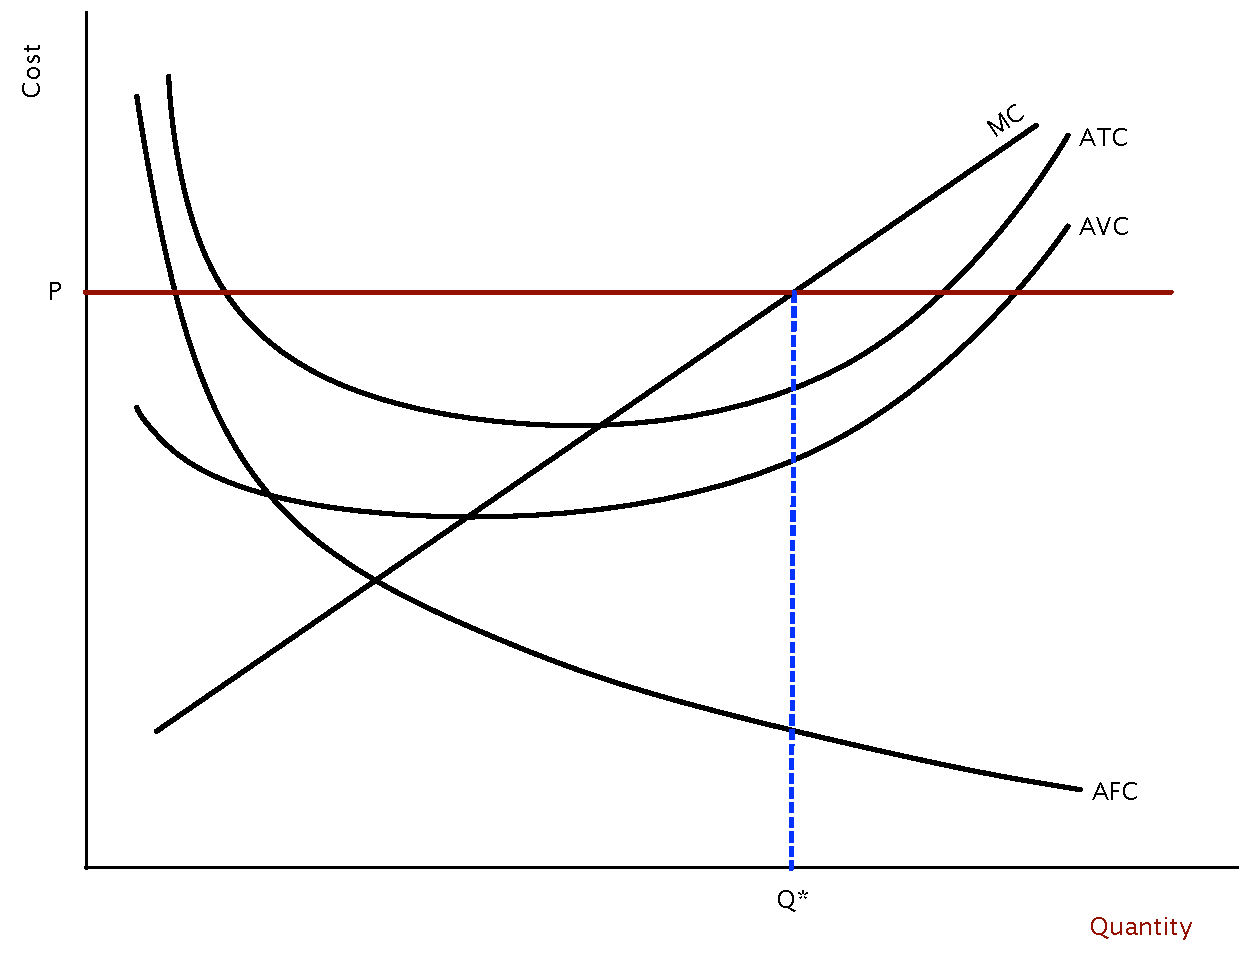
\includegraphics[scale=.35]{plot61.pdf}}
		\caption{Perfectly Competitive Environment}
	\end{figure}
	
\end{frame}

\begin{frame}{Profit Maximization - Graphic Approach}
\begin{itemize}
	\item The price line is \dd{horizontal} because the competitive firm is a price taker. 	
	\item Then, the quantity at which profit is maximized is found by tracing down from where the \dd{marginal costs} curve and the \dd{price line (demand curve)} intersect.
\end{itemize}
\end{frame}

\begin{frame}{Profit Maximization - Graphic Approach}
	\begin{itemize}

		\item If the quantity is below $Q^*$, then the marginal revenue is \dd{greater than} the marginal cost. Thus, by \dd{increasing} output, the firm can increase its profit. 
		\item If the quantity were above $Q^*$, then the marginal revenue is \dd{less than} the marginal cost. Thus, by \dd{decreasing} output, the firm can increase its profit. 
	\end{itemize}
\end{frame}

\begin{frame}{Profit Maximization - Graphic Approach}
\begin{itemize}
	\item Additionally, we can find profit from a graph. Rewrite profit as 
	
	\[\Pi = TR - TC = \ddp{PQ - TC = (P-ATC)\times Q}\]

	
	
\end{itemize}
\end{frame}

\begin{frame}{Profit Maximization - Graphic Approach}

		
		\begin{figure}[H]
			\centering
			\caption{Firm Profits}
			\begin{subfigure}{.45\textwidth}
				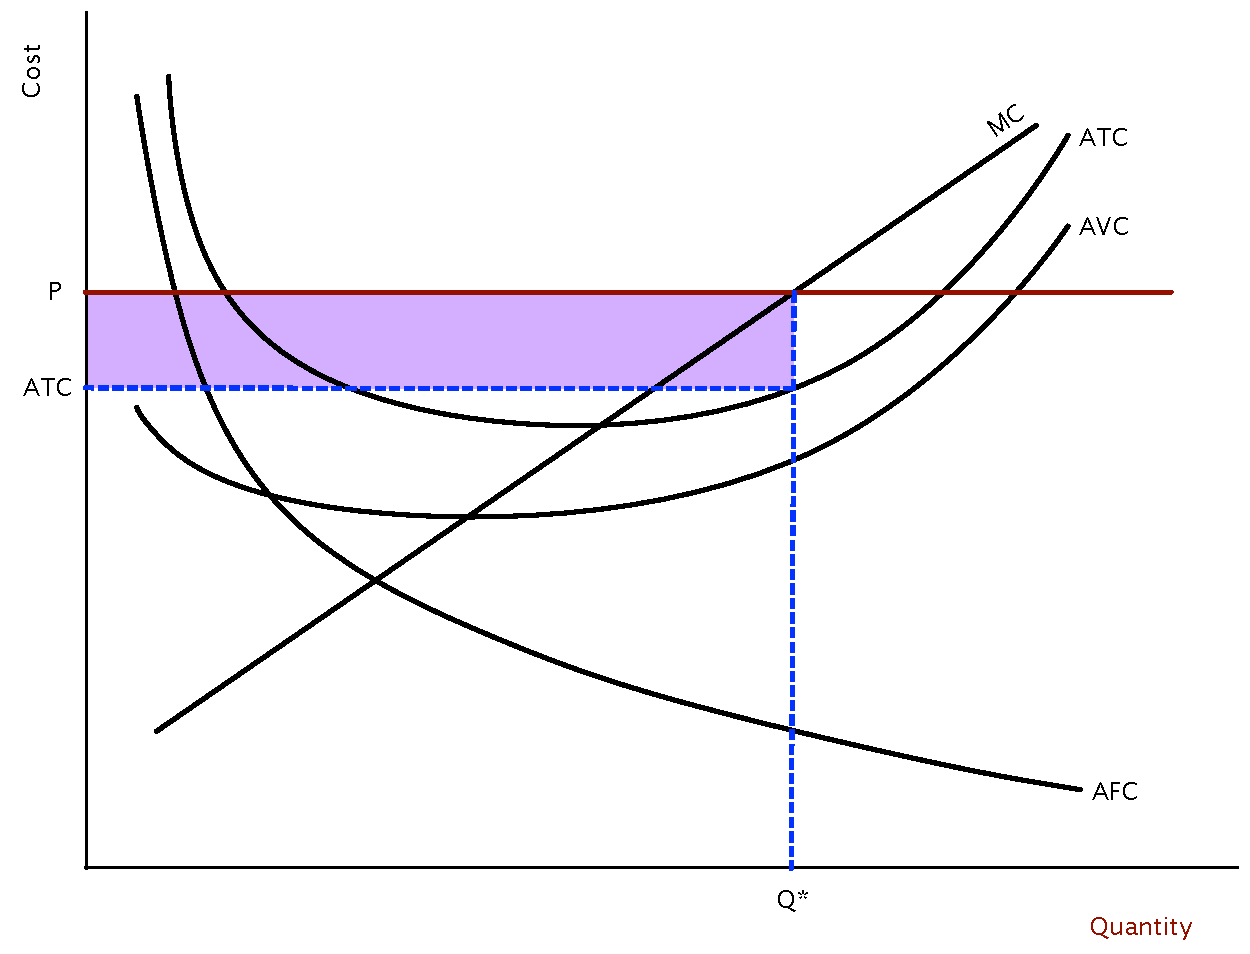
\includegraphics[scale=.2]{plot62.pdf}
				\caption{Firm Making Positive Profit}
			\end{subfigure}%
			\begin{subfigure}{.45\textwidth}
				\centering
				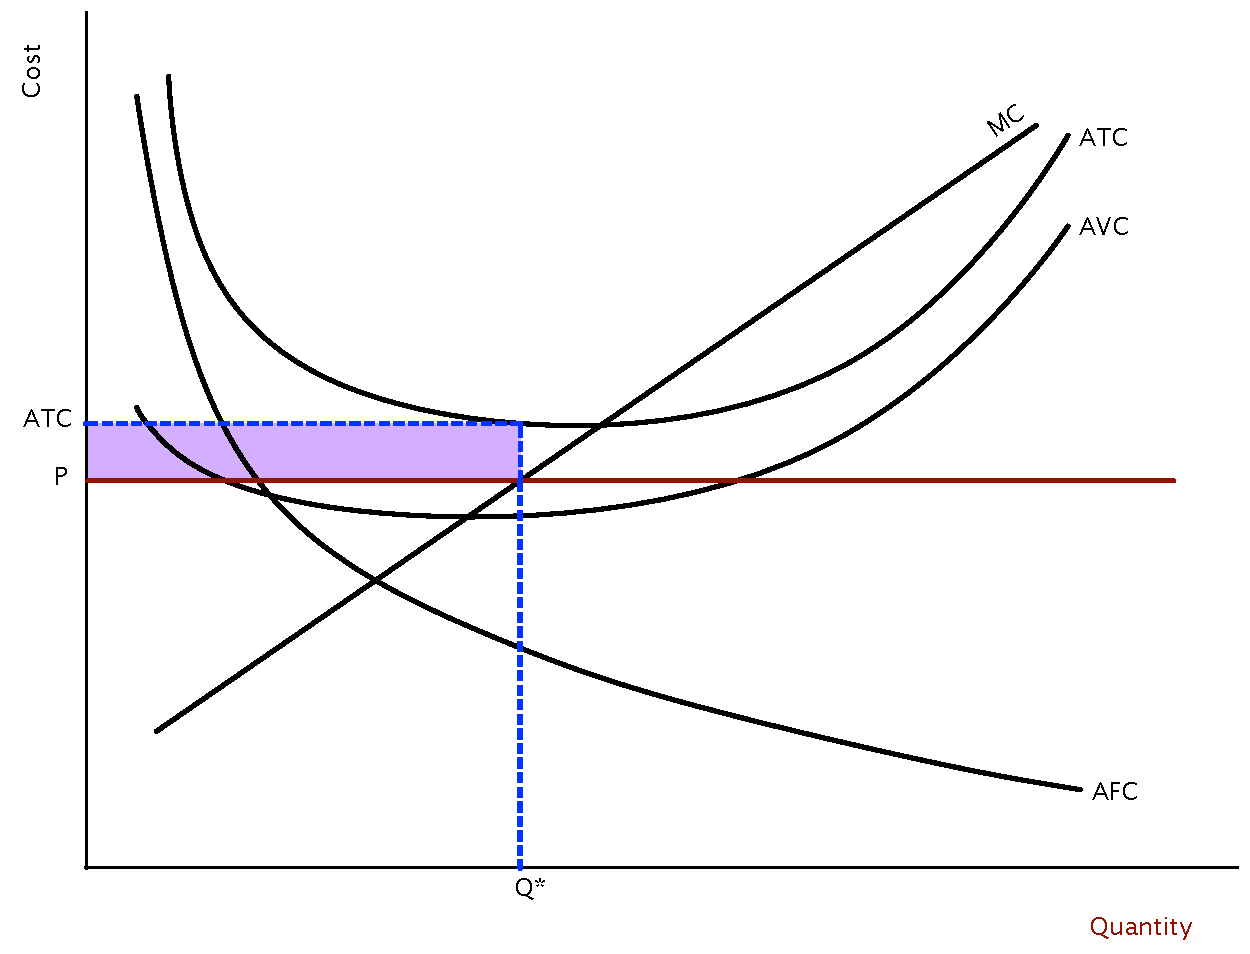
\includegraphics[scale=.2]{plot63.pdf}
				\caption{Firm Making Negative Profit}
			\end{subfigure}
		\end{figure}
		
\end{frame}

\section{Operating Decisions}

\begin{frame}{Short-Run Operating Decision}
\begin{itemize}
	\item \defn{Shutdown decision:} A \textit{short-run} decision to cease production during a specific period of time.
	\item 	In the short run, a firm's \dd{fixed costs} are sunk. Thus, when making its decision to produce in the short run, the firm only considers their \dd{variable costs}. 
\end{itemize}
\end{frame}

\begin{frame}{Short-Run Operating Decision}
	\begin{itemize}
		\item By shutting down, the firm would have a total revenue of \dd{\$0}. 
		\item But, it would not have to pay its variable costs (though it still has to pay its fixed costs). 
		\item Given this, the firm will only produce in the short run if \dd{$TR>VC$}. 
		\item \defn{Shut down rule:} \ddp{Shutdown if $ TR < TC \Rightarrow P < AVC$.}
		
	\end{itemize}
\end{frame}

\begin{frame}{Short-Run Operating Decision}
\begin{itemize}
	\item 	The portion of the $MC$ curve above the $AVC$ curve characterizes all the quantities at which a firm may produce. 
	\item This portion of the marginal cost curve is the firm's \dd{short-run supply curve}.
	

\end{itemize}
\end{frame}

\begin{frame}[b]{Short-Run Operating Decision}
		\begin{figure}[H]
			\centering
			\ddp{	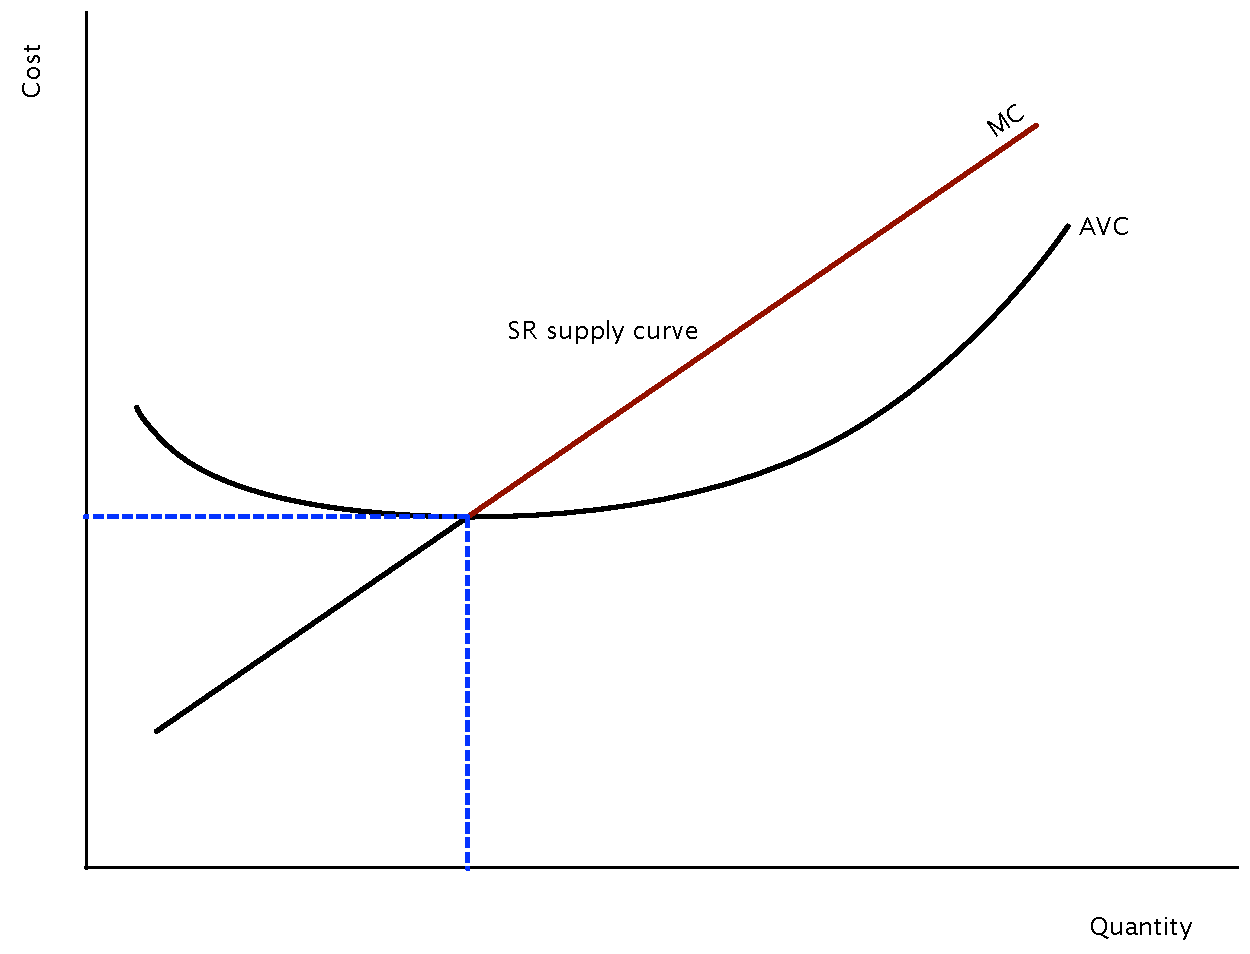
\includegraphics[scale=.3]{plot64.pdf}}
			\caption{Firm's Short-run Supply Curve}
		\end{figure}
		
\end{frame}

\begin{frame}{Short-Run Operating Decision}
	\begin{exmp} 
	Karlye's Klipz is a hair salon operating in a competitive market. The store's total costs each month are \$7,000. The salon has a yearly lease and pays \$3,000 each month in rent (part of the \$7,000 total monthly costs). All other costs change depending on how many haircuts are provided. The salon's haircuts are provided for \$25 each and they receive 175 patrons a month. What can you say about the salon's short-run decision? What will its profit be?
\end{exmp}
\pause \ddp{$FC = 3,000$, $VC = 4000$.\\
	 $AVC = 4000/175 = \$22.86 < P$, so stay open. \\
	 $\Pi = \$25 \times 175 - \$7,000 = -\$2,625.$ Profit if firms shuts down = -$\$3,000$.}
\end{frame}

\begin{frame}{Long-Run Exit Decision}
\begin{itemize}
	\item 	\defn{Exit decision:} A firm's \textit{long-run decision} to leave the market.
	\item In the long run, if the firm exits the market then (1) it loses all its revenue, but (2) it saves both its variable costs and fixed costs of production. 
	\item \defn{Exit rule:} \ddp{Exit if $TR < TC \Rightarrow P < ATC$}
	\item From the perspective of a party that wishes to enter the market, they will only do so if the venture will be profitable. Thus, a firm will only enter a market if \dd{$P > ATC$}.
\end{itemize}
\end{frame}

\begin{frame}{Long-Run Exit Decision}
\begin{itemize}
	\item The marginal cost curve above the average total cost curve characterizes the quantities the firm may produce if $P > ATC$. 
	\item This portion of the marginal cost curve is the firm's \dd{long-run supply curve}.

\end{itemize}
\end{frame}


\begin{frame}[b]{Long-Run Exit Decision}

		\begin{figure}[H]
			\centering
			\ddp{	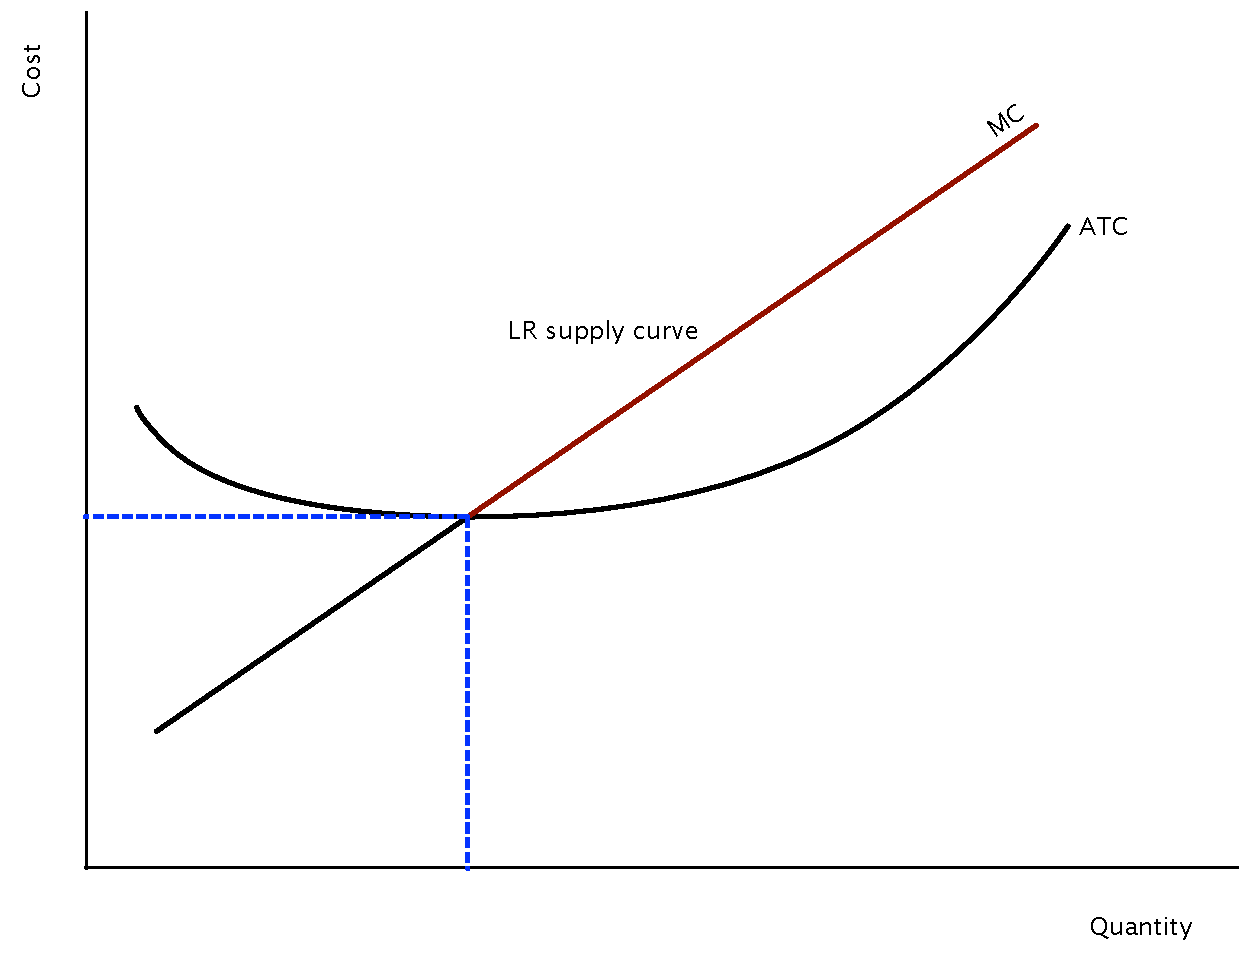
\includegraphics[scale=.3]{plot65.pdf}}
			\caption{Firm's Long-run Supply Curve}
		\end{figure}
		
		
\end{frame}

\begin{frame}{Long-Run Exit Decision}
	\begin{exmp}
	Consider Karlye's Klipz from Example 10.2. What can you say about the salon's long-run decision regarding exiting the market? 
\end{exmp}
\pause \ddp{$ATC = 7,000/175 = \$40 > P$, so exit in long run.}
\end{frame}

\section{Market Supply}

\begin{frame}{Market Supply in the Short-Run}
\begin{itemize}
	\item 	We saw how individual firms in a competitive market make optimal choices. How do these individual firms collectively form the supply curve for a market? 
	\item 	For any given price, each firm in a competitive market produces the quantity at which $P = MC$ (so long as $P > AVC$). 

\end{itemize}
\end{frame}


\begin{frame}{Market Supply in the Short-Run}
	\begin{itemize}
		\item To derive the market supply curve (in the short run), we add the individual short-run supply curves. 
		\item Since each firm is identical, the quantity supplied to the market at any given price is the quantity supplied by each firm times the number of firms in the market.
		
	\end{itemize}
\end{frame}

\begin{frame}{Market Supply in the Short-Run}
\begin{figure}[H]
	\centering
	\caption{Short-run Market Supply}
	\begin{subfigure}{.5\textwidth}
	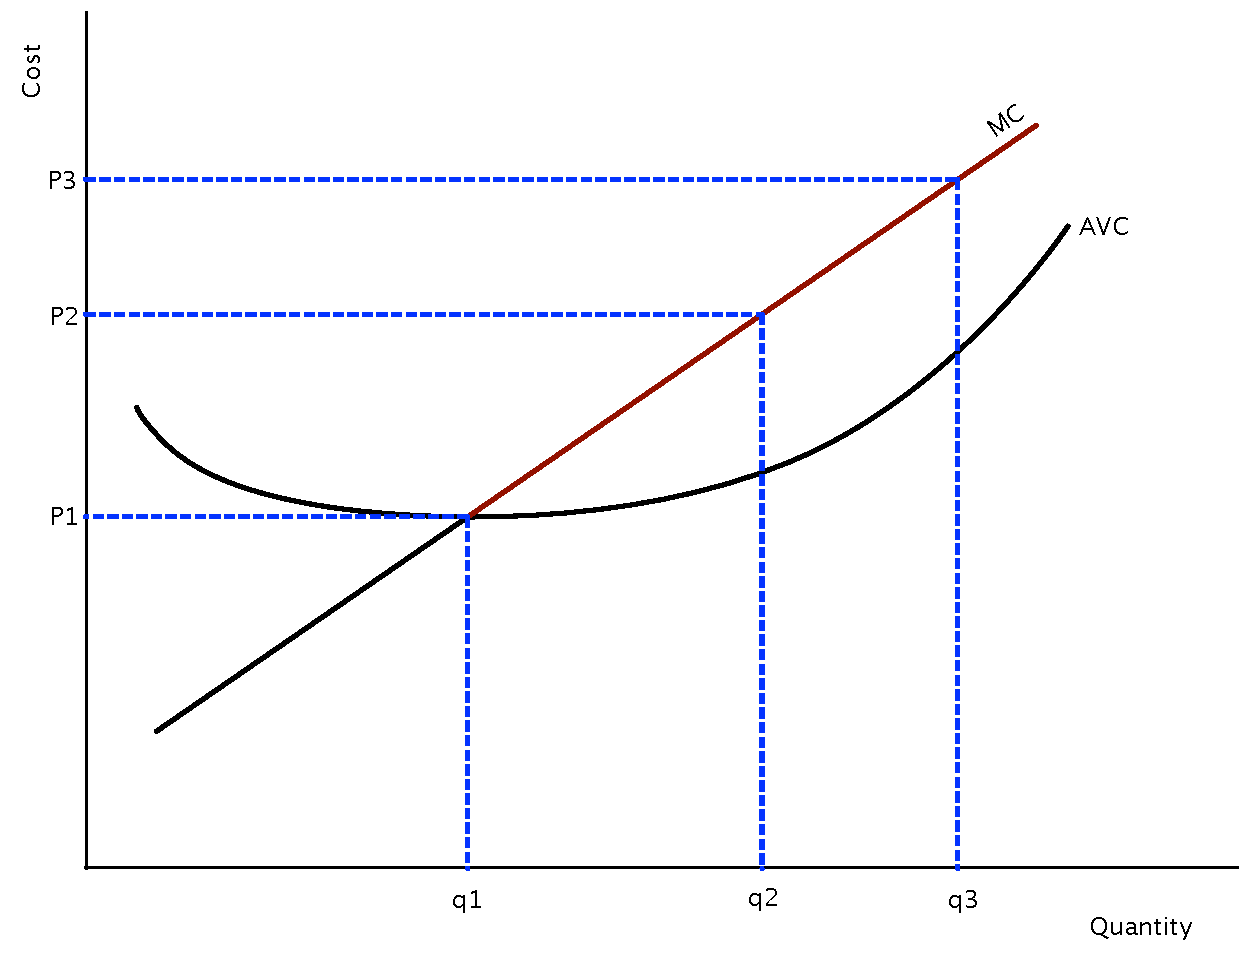
\includegraphics[scale=.25]{plot66.pdf}
		\caption{Individual Firm}
	\end{subfigure}%
	\begin{subfigure}{.5\textwidth}
		\centering
	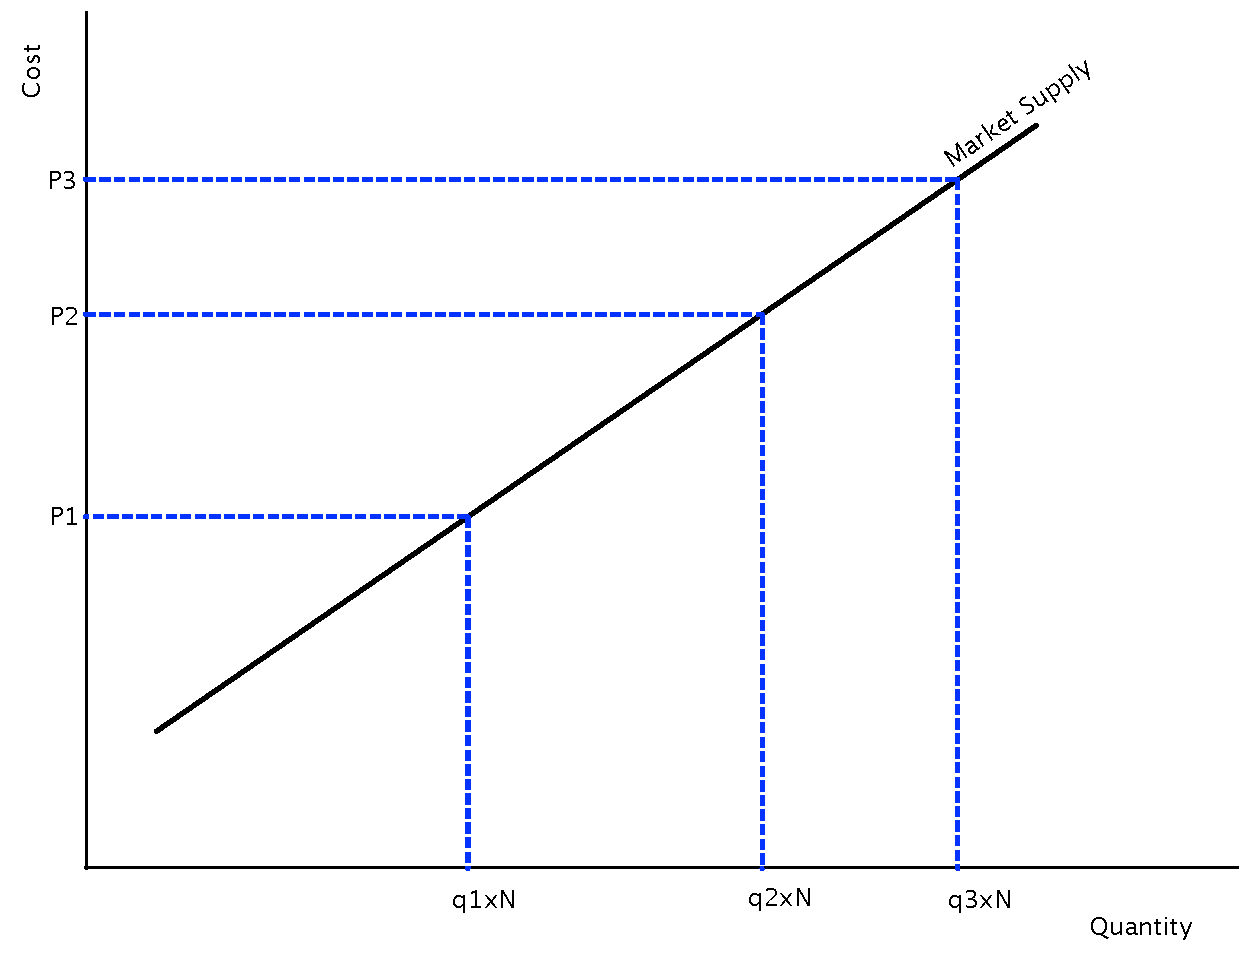
\includegraphics[scale=.25]{plot67.pdf}
		\caption{Market Supply}
	\end{subfigure}
\end{figure}

\end{frame}

\begin{frame}{Market Supply in the Long-Run}
\begin{itemize}
	\item 	In the long run, we assume that firms can freely enter and exit the market. If firms already in the market are profitable, then entrepreneurs outside the market will \dd{enter}. 
	\item This will \dd{increase} the number of firms in the market, which shifts the supply curve \dd{to the right}. 
	\item On the other hand, if firms in the market are not profitable, then they will exit the market. This shifts supply \dd{to the left}. 
	\item Finally, once this process finishes, the firms that do remain in the market make \dd{zero economic profit}, known as \dd{normal profit}.

\end{itemize}
\end{frame}

\begin{frame}{Market Supply in the Long-Run}
\begin{itemize}
	\item From the profit equation, $\Pi = (P - ATC) \times Q$, we see that firms producing output have zero profit if and only if $P = ATC$. 
	\item 	If firms in a competitive market set the quantity produced such that $P = MC$, and the process of entry \& exit implies that $P = ATC$, then it has to be that at $Q^*$, $MC = ATC$. 
	\item We know that if $MC = ATC$, then the firm has to be producing at the \dd{minimum} of ATC. 
	\item Thus, we have that firms in a competitive market will operate at their \dd{efficient scale} and \dd{$P = \min ATC$} in the long run.
\end{itemize}
\end{frame}

\begin{frame}{Market Supply in the Long-Run}
	\begin{exmp} Suppose that the market for donuts begins at its long-run equilibrium. Draw a graph showing the quantity a seller in the market would produce, the $MR$ at this quantity, the average total cost, and the firm's profit. Additionally, draw a graph showing the market for donuts. 
\end{exmp}



\end{frame}


\begin{frame}{Market Supply in the Long-Run}

	\begin{figure}[H]
		\centering
		\caption{Perfectly Competitive Market in Long-run}
		\begin{subfigure}{.35\textwidth}
			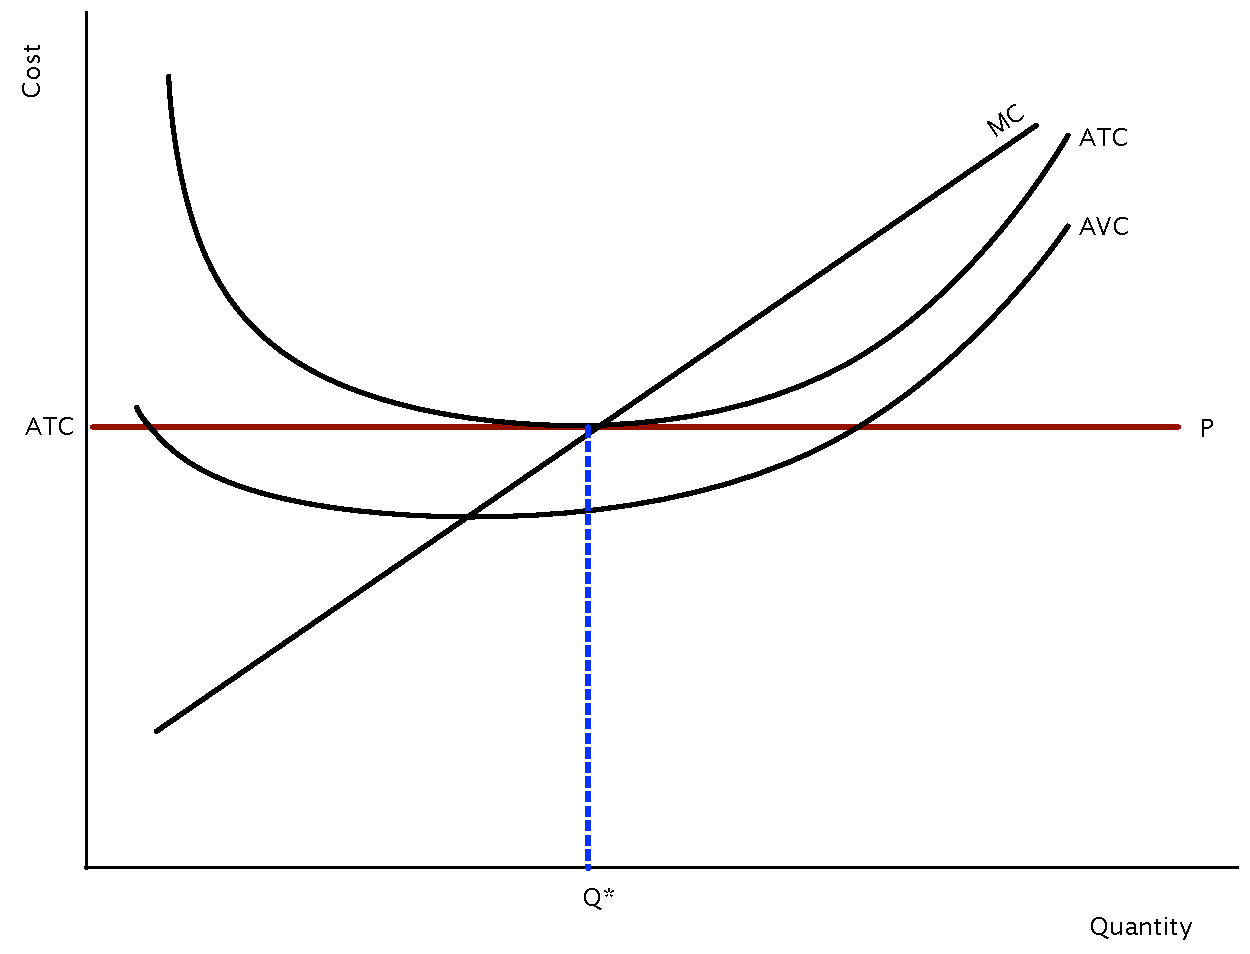
\includegraphics[scale=.2]{plot68.pdf}
			\caption{Individual Firm}
		\end{subfigure}%
		\begin{subfigure}{.35\textwidth}
			\centering
			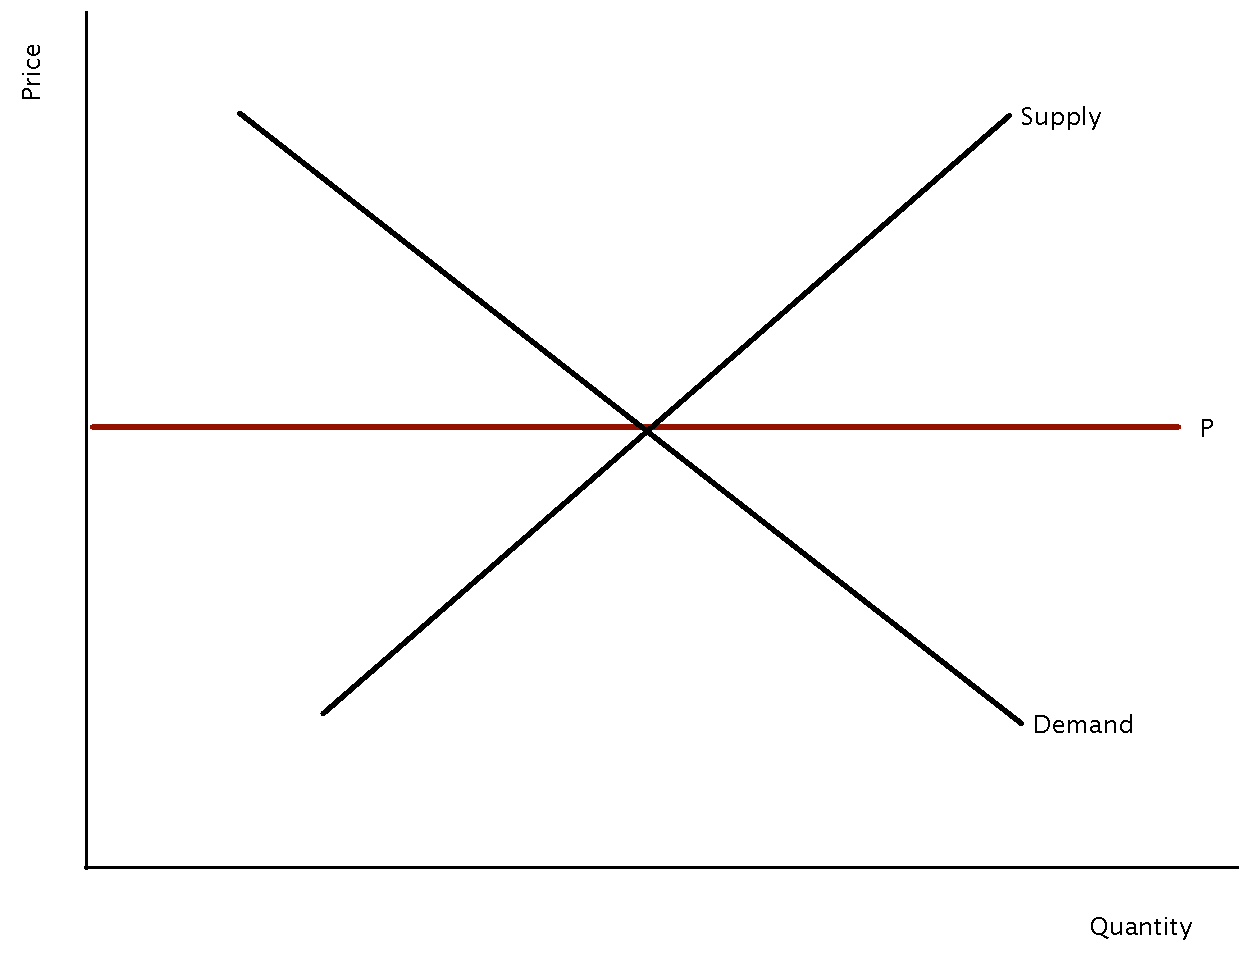
\includegraphics[scale=.2]{plot69.pdf}
			\caption{Market}
		\end{subfigure}
	\end{figure}
	
	
\end{frame}


\begin{frame}{Market Supply in the Long-Run}
\begin{exmp}
	Now, suppose the surgeon general announces that donuts cause severe health issues. What happens to the market price for donuts? How will firms in the market be affected in the short-run? In the long-run? Draw graphs to support your answers.
\end{exmp} 
\end{frame}



\begin{frame}{Market Supply in the Long-Run}
\begin{figure}
	\begin{subfigure}{0.35\textwidth}
		\centering
	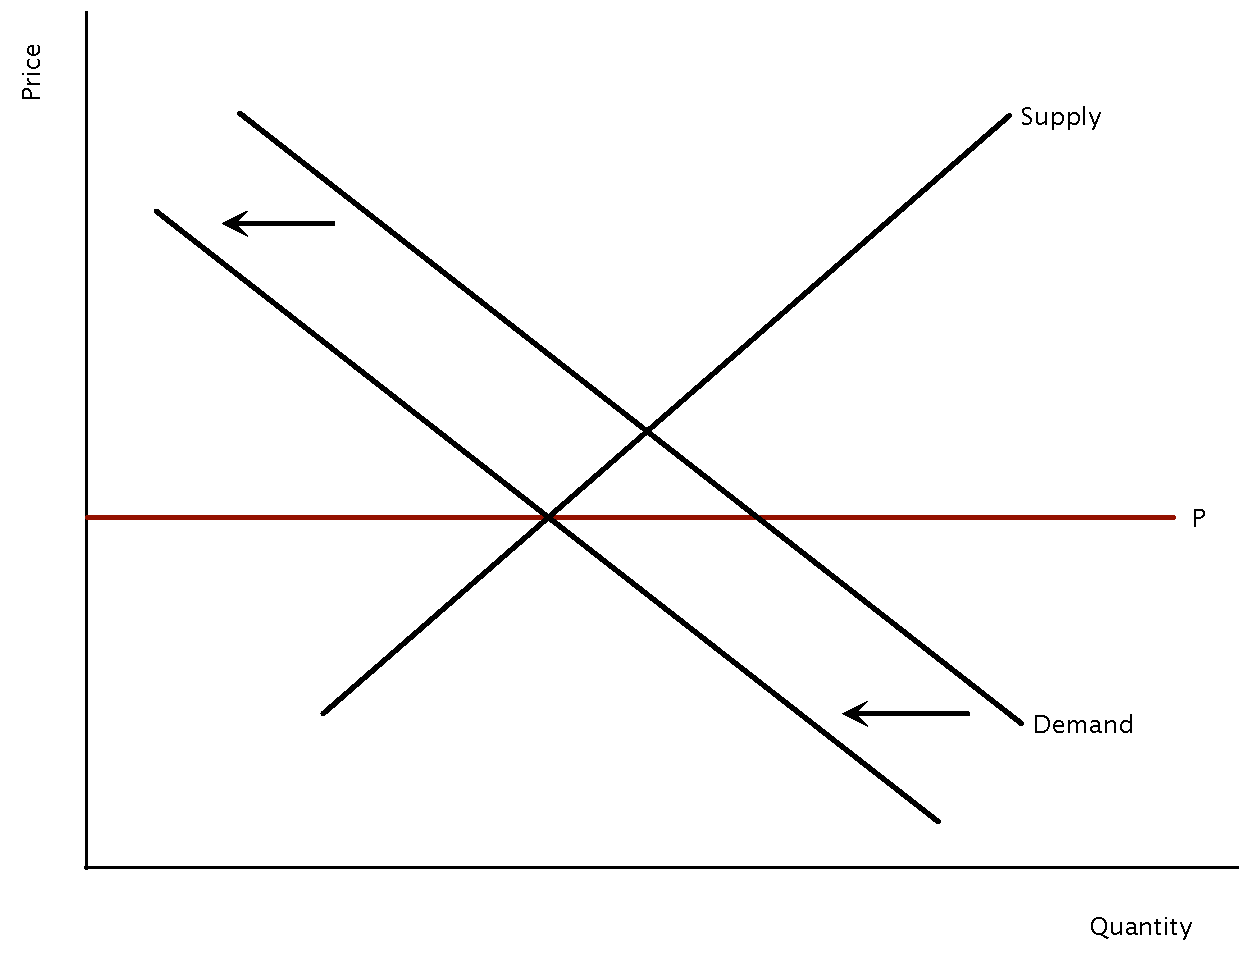
\includegraphics[scale=.2]{plot70.pdf}
		\caption{Market in SR}
	\end{subfigure}
	\begin{subfigure}{0.35\textwidth}
		\centering
		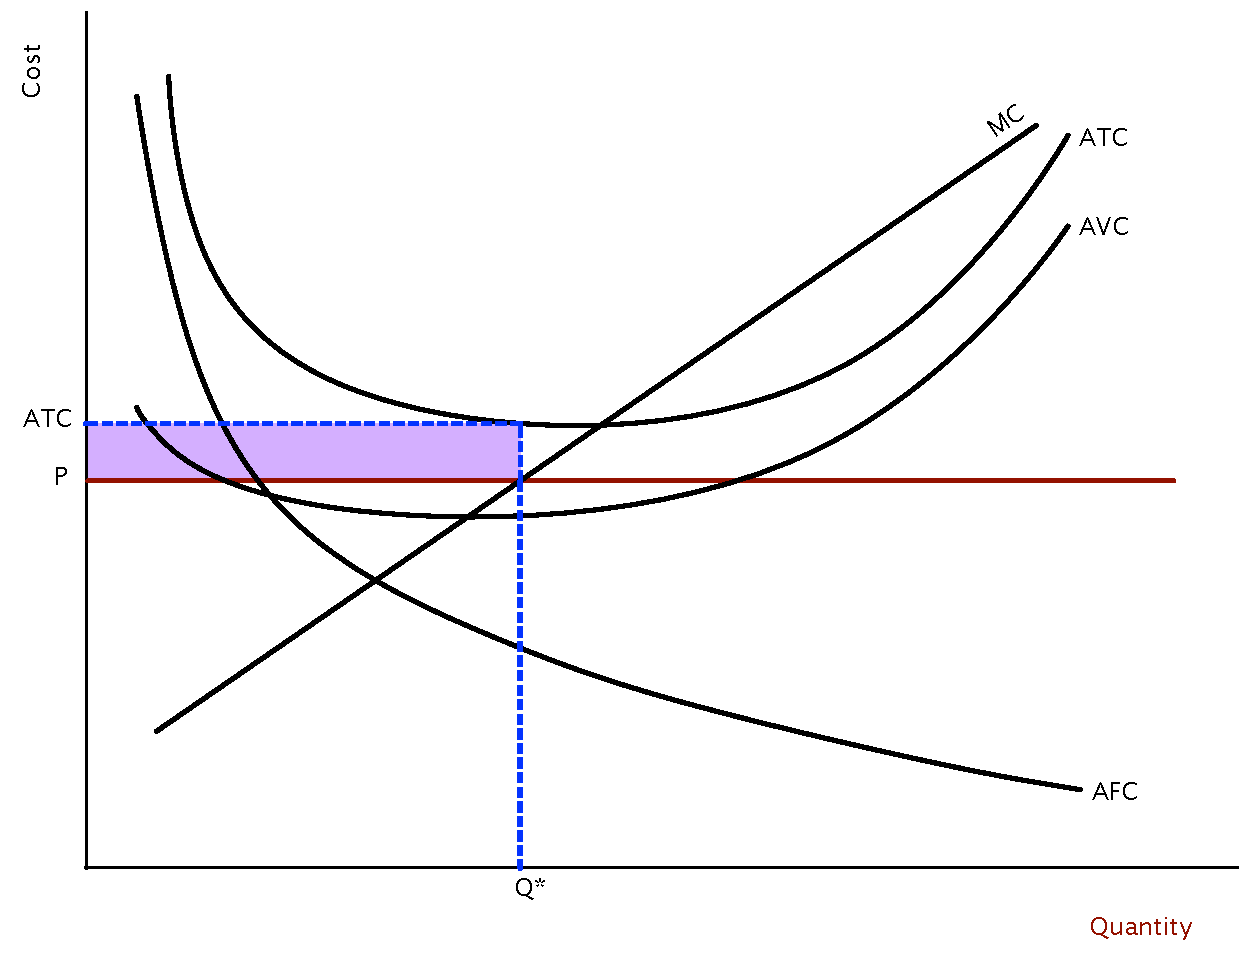
\includegraphics[scale=.2]{plot71.pdf}
		\caption{ Firms in SR}
	\end{subfigure}
\end{figure}

\end{frame}

\begin{frame}{Market Supply in the Long-Run}
	\begin{figure}
	\begin{subfigure}[b]{0.35\textwidth}
		\centering
		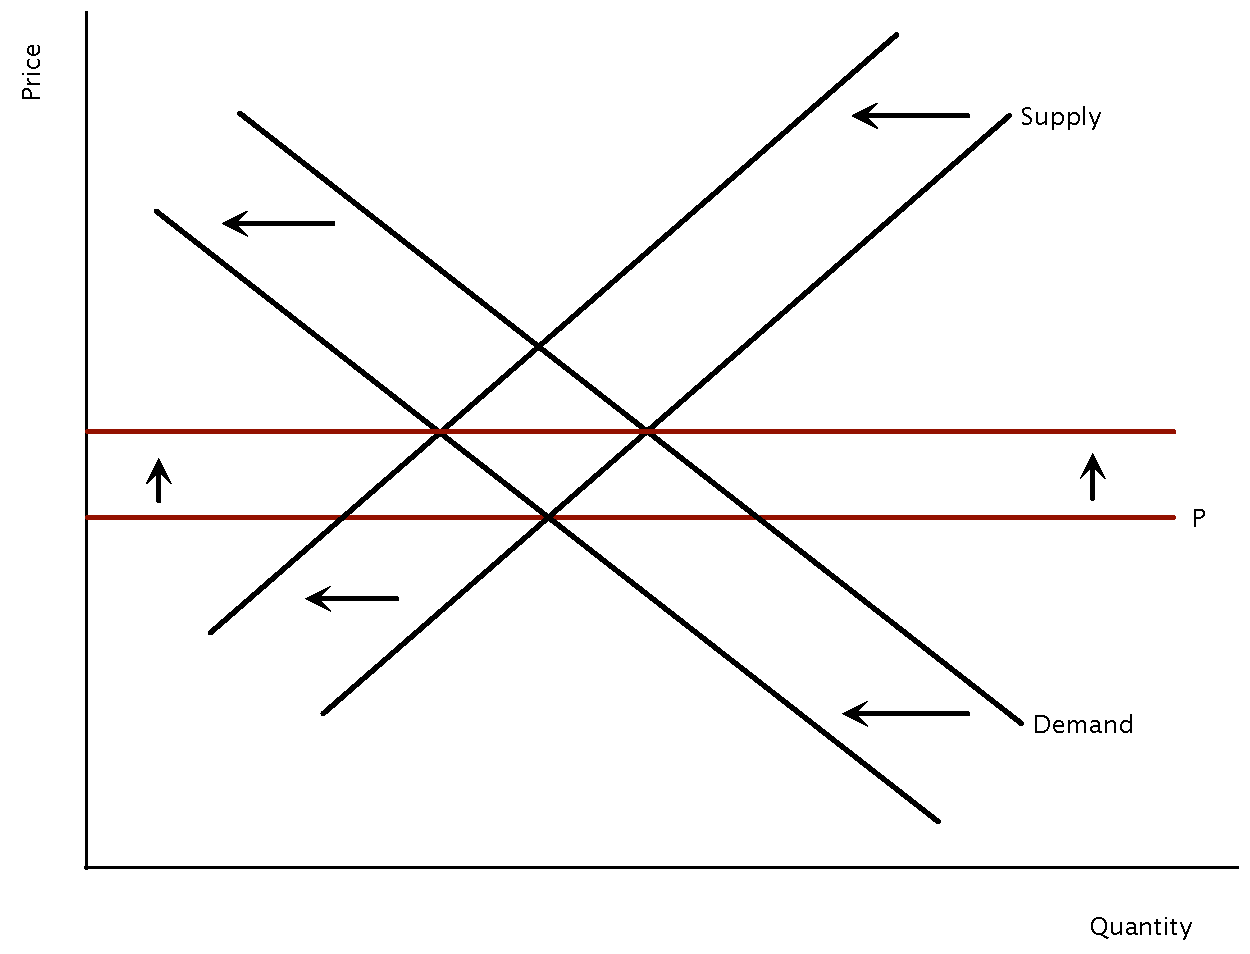
\includegraphics[scale=.2]{plot72.pdf}
		\caption{Market in Long-run}
	\end{subfigure}
	\begin{subfigure}[b]{0.35\textwidth}
		\centering
	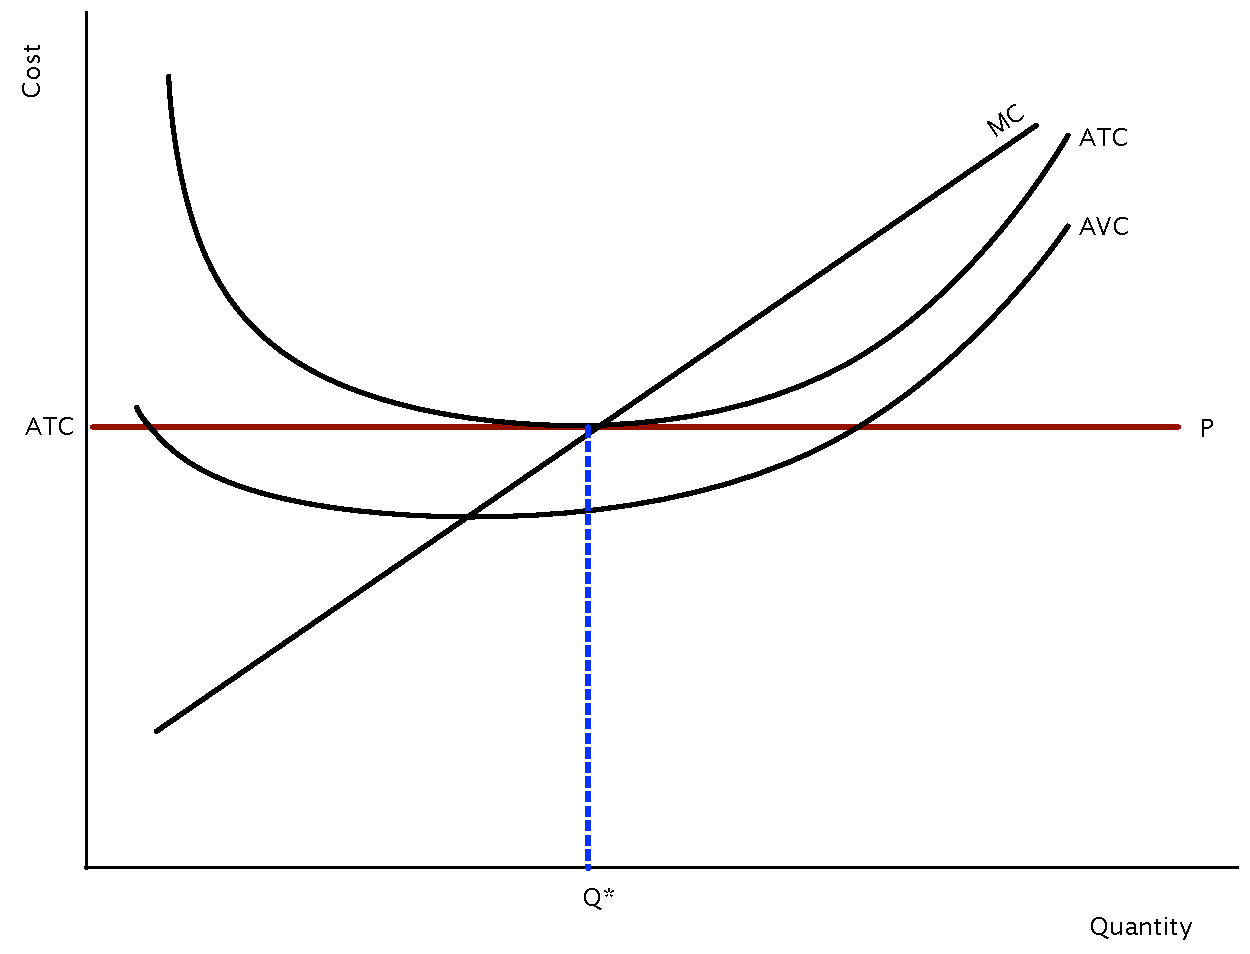
\includegraphics[scale=.2]{plot68.pdf}
		\caption{Individual Firms in LR}
	\end{subfigure}
\end{figure}
\end{frame}


\begin{frame}{Readings and Assignments}
\begin{itemize}
	\item Today: Mankiw Ch. 14
	\item Next time: Mankiw Ch. 15
	\item Problem Set 3, section 2
\end{itemize}
\end{frame}

\end{document}